
% xetex expected
\documentclass[xetex,professionalfont]{beamer}

% we want math
\usepackage{amsmath}

% fixes and extensions to amsmath
\usepackage{mathtools}

% additional math symbols
\usepackage{amssymb}

% good-looking fractions in text via \sfrac
\usepackage{xfrac}

% fix spaces after custom commands (see below for examples)
\usepackage{xspace}

% minted allows for fancy syntax highlighting (requires python with pygments)
% usage:
%   \begin{minted}{python}
%   codeb
%   \end{minted}
% \usepackage{minted}

% better looking tables
% usage:
%   begin with a \toprule, write a single row of column headings,
%   then add \midrule and after the columns of data we finish with \bottomrule
% example:
%   \begin{tabular}{llr} \toprule
%   Animal & Description & Price \midrule
%   cat & foo & 10 \\
%   dog & bar & 20 \\ \bottomrule
%   \end{tabular}
% note that good tables generally neither have vertical rules nor double rules
\usepackage{booktabs}

% system font support (requires xetex or luatex)
\usepackage{fontspec}
\setmonofont[Scale=0.7]{Cousine} % part of ttf-chromeos fonts on Arch

% improve microtypography
\usepackage{microtype}

% multi-language quotes for babel
\usepackage{csquotes}

% easy way to include copyright information
\usepackage{copyrightbox}

% better bibliographies
\usepackage[backend=biber,style=authoryear]{biblatex}

% language support (english,ngerman)
\usepackage[english]{babel}

% -----------------------------------------------------------------------------

% specify PDF metadata
\hypersetup{pdftitle={CVSP VO - Preview},pdfsubject={},pdfauthor={Christopher Pramerdorfer}}

% copyright font style
\makeatletter\renewcommand{\CRB@setcopyrightfont}{\tiny\color{lightgray}}

% make emph bold
\DeclareTextFontCommand{\emph}{\bfseries}

% add bib file
\addbibresource{literature.bib}

% use tuwcvl beamer theme
\usetheme{tuwcvl}

% -----------------------------------------------------------------------------

% common english abbreviations
\newcommand{\ie}{\mbox{i.e.}\xspace} % i.e.
\newcommand{\eg}{\mbox{e.g.}\xspace} % e.g.

% math - argmin and argmax
\DeclareMathOperator*{\argmin}{arg\,min}
\DeclareMathOperator*{\argmax}{arg\,max}

% shortcuts for number ranges
\newcommand{\NN}{\mathbb{N}}
\newcommand{\ZZ}{\mathbb{Z}}
\newcommand{\QQ}{\mathbb{Q}}
\newcommand{\RR}{\mathbb{R}}

% bold vectors
\renewcommand{\vec}[1]{\ensuremath{\mathbf{#1}}}

% vector shortcuts
\newcommand{\va}{\vec{a}}
\newcommand{\vb}{\vec{b}}
\newcommand{\vc}{\vec{c}}
\newcommand{\ve}{\vec{e}}
\newcommand{\vr}{\vec{r}}
\newcommand{\vs}{\vec{s}}
\newcommand{\vt}{\vec{t}}
\newcommand{\vu}{\vec{u}}
\newcommand{\vv}{\vec{v}}
\newcommand{\vw}{\vec{w}}
\newcommand{\vx}{\vec{x}}
\newcommand{\vy}{\vec{y}}
\newcommand{\vz}{\vec{z}}

% -----------------------------------------------------------------------------

\title{Computer Vision Systems Programming VO}
\subtitle{Introduction}
\author{Christopher Pramerdorfer}
\institute{Computer Vision Lab, Vienna University of Technology}

\begin{document}

% -----------------------------------------------------------------------------

\begin{frame}
\maketitle
\end{frame}

% -----------------------------------------------------------------------------

\begin{frame}
\frametitle{Lecture Topics}

Computer Vision (CV) software and resources\\\medskip
Models vs.\ algorithms\\\medskip
CV applications with commercial success

\bigskip
\begin{center}
	\copyrightbox[b]
	{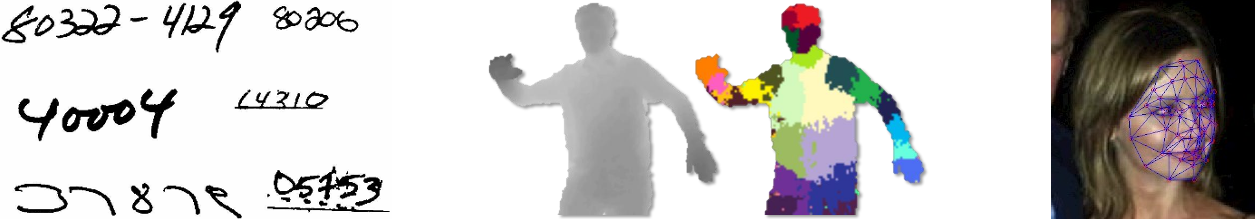
\includegraphics[width=10cm]{figures/intro-collage.png}}
	{\centering Images from \cite{lecun1989}, \cite{shotton2011}, \cite{taigman2013}}
\end{center}

\end{frame}

% -----------------------------------------------------------------------------

\begin{frame}
\frametitle{Lecture Topics}
\framesubtitle{Computer Vision Software and Resources}

Programming languages and libraries
\begin{itemize}
	\item Matlab
	\item Python (SciPy, scikits, ...)
	\item C++ (OpenCV, Shark, Caffe, ...)
\end{itemize}

\bigskip
Programming resources (throughout lecture)
\begin{itemize}
	\item Code snippets, weblinks
\end{itemize}

\end{frame}

% -----------------------------------------------------------------------------

\begin{frame}
\frametitle{Lecture Topics}
\framesubtitle{Models vs. Algorithms}

How to approach CV problems systematically
\begin{itemize}
	\item Difference between models and algorithms
	\item How to model and solve CV problems
	\item Numerical optimization
\end{itemize}

\end{frame}

% -----------------------------------------------------------------------------

\begin{frame}
\frametitle{Lecture Topics}
\framesubtitle{Selected CV Applications}

CV applications with commercial success
\begin{itemize}
	\item Face detection and panorama stitching in cameras
	\item Player pose estimation from 3D data for gaming (Kinect)
	\item Face and object recognition
\end{itemize}

\bigskip
We will see
\begin{itemize}
	\item How they work
	\item How they are implemented
\end{itemize}

\end{frame}

% -----------------------------------------------------------------------------

\begin{frame}
\frametitle{Lecture Location and Schedule}

\textbf{Location}: Seminarraum 183/2, Favoritenstr. 9\\
\textbf{Time}: Wed 10:15 -- 11:45 s.t.

\bigskip
\textbf{Schedule}: \url{http://www.caa.tuwien.ac.at/cvl/teaching/wintersemester/cvsp_vo/index.html}

\bigskip
Follow \texttt{@tuwcvsp} on Twitter for updates

\end{frame}

% -----------------------------------------------------------------------------

\begin{frame}
\frametitle{Prerequisites}

Basic image processing and computer vision knowledge
\begin{itemize}
	\item What is linear filtering?
	\item What is a camera matrix?
\end{itemize}

\bigskip
Some knowledge of probability is recommended
\begin{itemize}
	\item What is a normal distribution?
	\item What is Bayes' rule?
\end{itemize}

\end{frame}

% -----------------------------------------------------------------------------

\begin{frame}
\frametitle{Grading}

There will be an oral exam (about 15 minutes)

\bigskip
Dates will be posted on \url{http://www.caa.tuwien.ac.at/cvl/teaching/wintersemester/cvsp_vo/index.html}

\end{frame}

% -----------------------------------------------------------------------------

\begin{frame}
\frametitle{Associated Lab Exercise}

We recommend the associated lab exercise to
\begin{itemize}
	\item Explore a CV topic of your choice in more detail
	\item Get used to software covered in this lecture
\end{itemize}

\end{frame}

% -----------------------------------------------------------------------------

\begin{frame}
\frametitle{Bibliography}

\printbibliography

\end{frame}

\end{document}